\documentclass{article}
\usepackage[UTF8]{ctex}
\usepackage{float}
\usepackage{graphicx}

\title{项目作业:五则运算计算器的实现}
\author{林敬翊}
\date{2022年12月31日}

\begin{document}

\maketitle

\section{设计思路}
在设计此程序时,刚开始我先用void程序把程序可能报错的原因写出来,方便后面报错时直接把该原因弹出,并且直接退出运行.\par
接下来输入用$int\,Priority$函数,根据数学的规则分辩他们的优先级,指数优先,在到乘除,最后才是加减。 \par
然后在使用$int\,Operator$函数,为接下来的运算做铺垫。\par
再来开始到我们的重头戏,也就是计算的前后顺序。这里我们使用$void\,CalculatorFunction$ 通过判断$for$循环,依次辨别每一个输入的字。对应的符号根据对应的规则利用$stack$和$vector$的操作,并且归类好。 \par
接着我们就到$void\,cal$为了方便等下$void\,calculate()$ 的计算。\par
最后就是$void\,calculate()$ ,里面记载了所有+\quad-\quad*\quad/\quad \^{} 的计算方法,在有前面的归类后,这里运算就变得特别简单
\section{测试结果}
课程作业里面的测试数据与结果为(图1):\par
2\^{}(1+3)-5*(15.23)/(1 + 2)*3-5 \par
1.25+(3*(1+2\^{}2)*3-43)\^{}(4-2) \par
2\^{}(1+3))-5*(15.23)/(1+2)*3-5\par
2\^{}(1+3)-5*(15.23)/(1-1)*3-5\par
\begin{figure}[H]
		\centering
		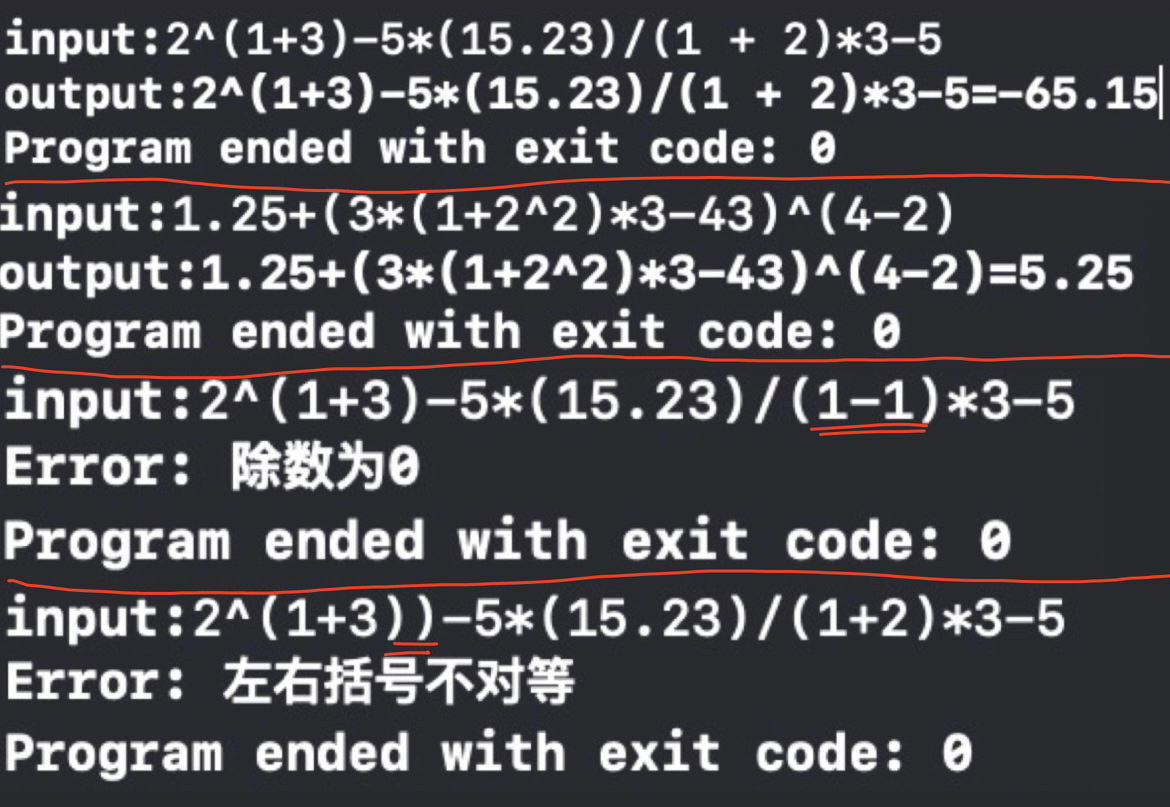
\includegraphics[scale=0.21]{test pic1.png}	
            \caption{以上为项目作业测试对应结果}
\end{figure}\par
测试数据与结果为(图2):\par
\^{}(1+3)-5*(15.23)/(1-1)*3-5\par
1.25+(3*(1+2\^{}2)*3-43)\^{}(4-2)+-3\par
" " \par
2\^{}(1+3)-5*(15.23)/(1 + 2)*3-5a\par
\begin{figure}[H]
		\centering
		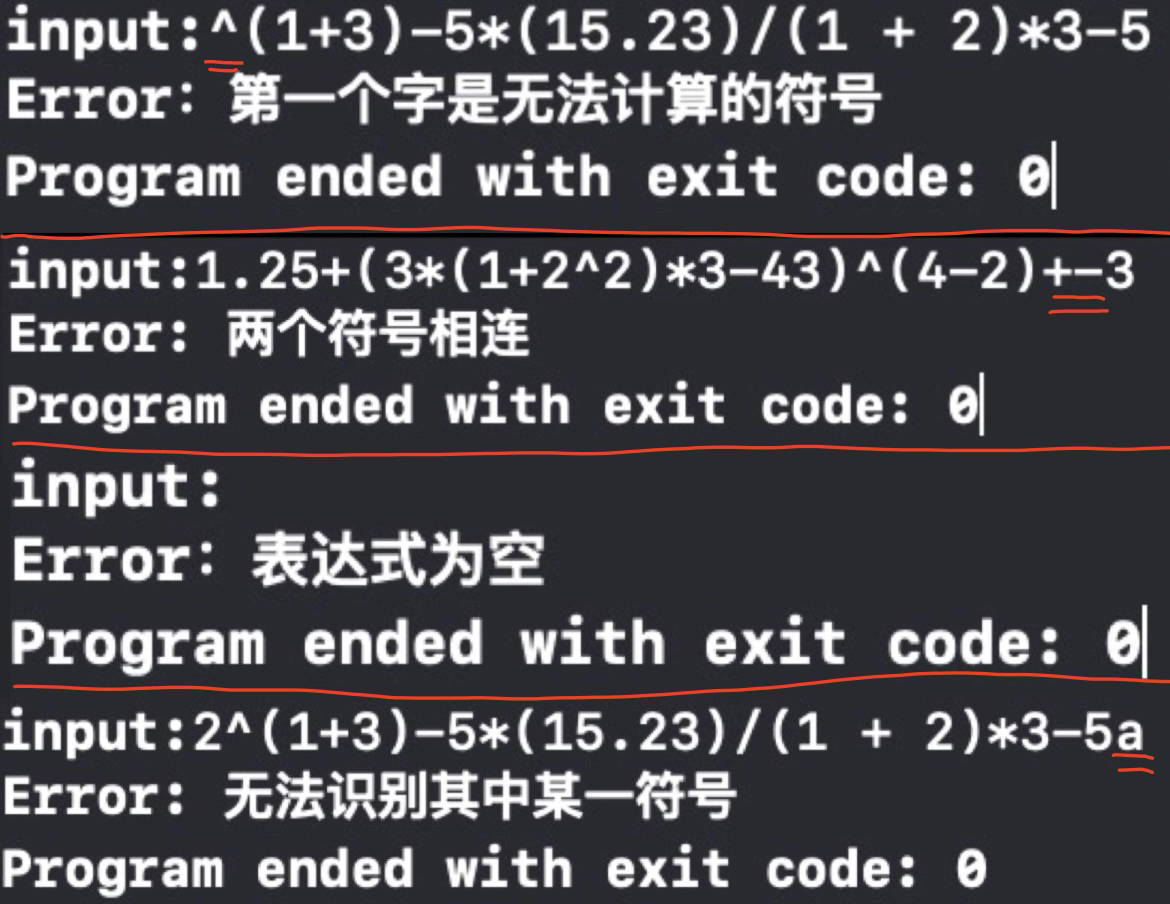
\includegraphics[scale=0.21]{test pic2.png}	
            \caption{自行测试对应结果}
\end{figure}\par



\end{document}
